\subsection{综合证明与例题：存在性、识别与比较静态}

\subsection{一个完整的参数化例子}
考虑 $B(p,w)=\{x\in\mathbb R_+^2:p_1x_1+p_2x_2\le w\}$ 与
$u(x)=\min\{x_1,2x_2\}$。由于效用是凹函数，最优点位于 $x_1=2x_2$ 与预算线的交点，故
\[
x_1^*=\frac{2w}{p_1+2p_2},\qquad x_2^*=\frac{w}{p_1+2p_2},\qquad
v(p,w)=\frac{w}{p_1+2p_2}.
\]
该例展示：偏好结构先决定等效用线的形状，约束再决定可实现的切点。

\begin{figure}[H]\centering
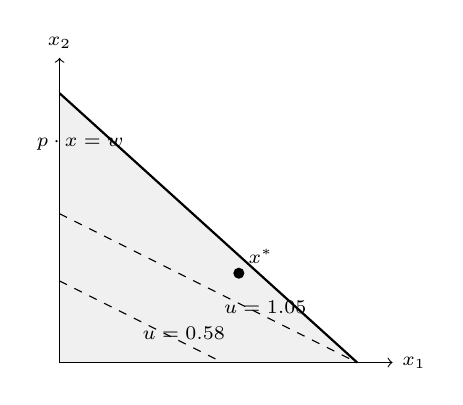
\begin{tikzpicture}[x=0.9cm,y=0.9cm,font=\scriptsize]
\fill[gray!12] (0,0)--(0,3.8)--(4.2,0)--cycle;
\draw[->] (0,0)--(4.7,0) node[right] {$x_1$};\draw[->] (0,0)--(0,4.3) node[above] {$x_2$};
\draw[thick] (0,3.8)--(4.2,0) node[pos=.25,above left] {$p\cdot x=w$};
\draw[dashed] (0,2.1)--(4.2,0) node[pos=.52,below right] {$u=1.05$};
\draw[dashed] (0,1.15)--(2.3,0) node[pos=.45,below right] {$u=0.58$};
\fill (2.53,1.26) circle (2pt) node[above right] {$x^*$};
\end{tikzpicture}
\caption{完美互补偏好的最优点}
\end{figure}
\figexplan{两条虚线是 L 形偏好的等效用线的斜段示意，预算边界与最高可达等效用线在比例固定的点相交。最优解不是切线条件，而是固定比例条件与预算约束共同决定。}

\subsection{比较静态的符号判断}
由 $v=w/(p_1+2p_2)$，有 $\partial v/\partial w>0$、$\partial v/\partial p_i<0$。当 $p_1$ 上升时，$x_1^*$ 和 $x_2^*$ 均下降，原因是该例中两种商品严格互补。与之相比，替代品模型可能出现交叉价格效应为正；因此不能仅凭预算收缩判断每个分量的方向。

\subsection{存在性与唯一性的逻辑分离}
Weierstrass 定理只保证最大值被达到，不保证唯一性。严格拟凹性保证最优集合至多一个点；一般拟凹性允许一段最优点；非拟凹性甚至可能有多个分离的局部峰。研究写作中必须分别报告“存在”“唯一”和“可微”，三者是不同结论。

\begin{table}[H]\centering\small
\begin{tabular}{p{3cm}p{4cm}p{4cm}}
\toprule
条件 & 可推出什么 & 不能推出什么\\
\midrule
连续 $u$，紧 $B$ & 最优解存在 & 不保证唯一、可微\\
严格拟凹 & 最优解唯一（若存在） & 不保证闭式解\\
二阶可微 & 可用 Hessian 检验局部性质 & 不自动保证全局最优\\
严格凸约束集 & 几何结构更规整 & 不替代目标函数的凹性\\
\bottomrule
\end{tabular}
\caption{最优性结论的条件分层}
\end{table}

\subsection{综合练习}
\begin{enumerate}
\item 证明预算集在 $p\gg0$、$w<\infty$ 时紧。
\item 对 $u=x_1^\alpha x_2^{1-\alpha}$ 推导 Marshall 与 Hicks 需求，并验证 Slutsky 对称性。
\item 构造一个连续但非拟凹的效用函数，说明一阶条件可能产生多个候选点。
\item 解释为什么相同的选择预测并不意味着相同的福利判断。
\end{enumerate}
